
\chapter{Methodology}
\section{ Project Management Model}

Our project began with a comprehensive requirements gathering phase where we collaborated closely with the client to define the project's scope. We established a set of core features for a Minimum Viable Product (MVP) \cite{atlassian_mvp}, which was formally documented and approved. This clear initial plan allowed us to structure the project efficiently while also outlining a roadmap for future enhancements. A key objective was to minimize dependencies among team members. To achieve this, we created a well-structured Product Requirements Document (PRD) \cite{atlassian_requirements} that enabled each team member to work on different components independently, fostering a parallel development process and ensuring a clear understanding of individual responsibilities.

\begin{figure}[h]
    \centering
    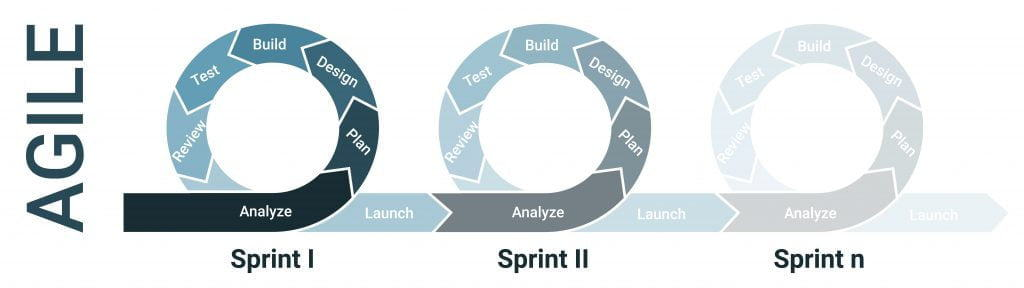
\includegraphics[width=0.8\textwidth]{agile.jpeg}
    \caption{Agile Methodology}
    \label{fig:agile}
\end{figure}

Given our need for flexibility and continuous client engagement, we adopted the Agile methodology \cite{atlassian_agile} as our primary project management framework. This approach allowed us to break down the project into manageable iterations, or sprints, rather than adhering to a rigid, linear timeline. To facilitate this, we leveraged Jira \cite{atlassian_jira}, a powerful project management tool. Jira enabled us to create and assign tasks, manage our sprints, and conduct thorough sprint reviews. This process provided our team with clear visibility into the development pipeline and ensured that we were consistently delivering value. Furthermore, we integrated a Continuous Integration (CI)\cite{atlassian_ci}. This allowed us to automate the building, testing, and deployment of our code, ensuring that new features and bug fixes could be released efficiently and reliably. This combination of an Agile workflow, supported by Jira and automated through CI, allowed us to maintain a dynamic and responsive development process that could quickly adapt to new requirements and feedback.

% Our team operated with an independent, decentralized structure where each member took ownership of their assigned tasks. This platform provided a transparent view of our progress and allowed us to manage our workload effectively. Our team maintained a consistent communication cadence with weekly meetings every Monday to review sprint progress, address any roadblocks, and plan the upcoming week's tasks. Furthermore, we held meetings with the client every Friday, which served as dedicated sessions for feature demos, gathering feedback, and addressing any questions or new requests. To tackle complex tickets that required collaborative effort, we also adopted pair programming on other weekdays. This practice not only facilitated the resolution of challenging technical issues but also promoted knowledge sharing and code quality across the team.

\section{Software Development Lifecycle}
% The backend for the project, a Multilingual Virtual Tour Assistant for Local Navigation (MTAP), is a microservices-based system designed for scalability and robustness. Built primarily with Java 21 and the Spring Boot framework, the architecture emphasizes loose coupling and domain-driven design. The system is comprised of several key services, including an API Gateway to handle routing and security, Location-based data, Translation, Navigation, and Content management. The project uses PostgreSQL for its primary database, Redis for caching, and Elasticsearch for efficient searching of points of interest. Continuous integration and deployment are managed through GitHub Actions. This combination of technologies and architectural patterns ensures the backend is both highly performant and easy to maintain.
    
\section{Technologies and Tools}
    \subsection{Programming Languages}
    \subsection{Frameworks and Libraries}
    \subsection{Databases}
    \subsection{Version Control}
    
% The frontend was built with a modern and scalable technology stack. Next.js was used as the primary framework, built on top of React, with TypeScript for strong typing. For styling and design, the team implemented Tailwind CSS with a Daisy UI. 
% React Context API was chosen for managing global state, such as user preferences and language settings, while React Query was utilized for handling server-side data, including caching and synchronization. For authentication, the project used NextAuth.js. The multilingual functionality was powered by next-i18next. These services include a User Service for profile management, a Location Service for nearby points of interest and navigation, and a Translation Service for dynamic content. For mapping, the project initially used Leaflet.js with OpenStreetMap.

\section{Data Collection and Analysis}
    \subsection{Data Sources}
    \subsection{Data Processing}
    
